%% =====================================================================
%% Control Valve Sizing Assignment - LAA01AA202
%% Layout follows the JAMK reporting template (Other_reporting_template.dotx):
%%   cover page with JAMK logos, sans-serif 12 pt, line spacing 1.5,
%%   margins 2 cm, page number top right, Contents/Figures/Tables on one page,
%%   captions above figures and tables, "Note." below, References, Appendices.
%%
%% STILL OPEN (marked red in the PDF):
%%  1. Optional: set DPm = 0.97 in Nelprof (gear icon at the charts),
%%     replace the installed charts and update Section 5.6.
%%  2. Proofread the AI declaration - it must describe what YOU really did.
%% =====================================================================
\documentclass[12pt,a4paper]{article}

% ----- Encoding, language, font -----
\usepackage[utf8]{inputenc}
\usepackage[T1]{fontenc}
\usepackage[english]{babel}
% Template font is Aptos (sans serif) -> closest free sans-serif font
\IfFileExists{tgheros.sty}{\usepackage{tgheros}}{\usepackage[scaled=0.92]{helvet}}
\renewcommand{\familydefault}{\sfdefault}

% ----- Layout -----
\usepackage[a4paper,margin=2cm,headheight=15pt,headsep=0.8cm]{geometry}
\usepackage{setspace}
\onehalfspacing
\setlength{\parindent}{0pt}
\setlength{\parskip}{10pt plus 2pt minus 1pt}
\emergencystretch=3em

% ----- Packages -----
\usepackage{graphicx}
\usepackage{xcolor}
\usepackage{amsmath}
\usepackage{amssymb}
\usepackage{booktabs}
\usepackage{tabularx}
\usepackage{float}
\usepackage{enumitem}
\usepackage{etoolbox}
\usepackage{titlesec}
\usepackage[titles]{tocloft}
\usepackage{caption}
\usepackage{fancyhdr}
\usepackage{tikz}
\usetikzlibrary{arrows.meta,calc,decorations.pathreplacing}
\usepackage{xurl}
\usepackage[hidelinks]{hyperref}
\urlstyle{same}
\Urlmuskip=0mu plus 1mu\relax

% ----- Headings as in the template (16 / 14 / 12 pt, bold, numbered) -----
\titleformat{\section}{\normalfont\fontsize{16}{19}\selectfont\bfseries}{\thesection}{0.8em}{}
\titleformat{\subsection}{\normalfont\fontsize{14}{17}\selectfont\bfseries}{\thesubsection}{0.8em}{}
\titleformat{\subsubsection}{\normalfont\normalsize\bfseries}{\thesubsubsection}{0.8em}{}
\titlespacing*{\section}{0pt}{18pt}{12pt}
\titlespacing*{\subsection}{0pt}{14pt}{8pt}
\titlespacing*{\subsubsection}{0pt}{12pt}{6pt}

% ----- Header: page number top right only -----
\pagestyle{fancy}
\fancyhf{}
\fancyhead[R]{\thepage}
\renewcommand{\headrulewidth}{0pt}
\fancypagestyle{plain}{\fancyhf{}\fancyhead[R]{\thepage}\renewcommand{\headrulewidth}{0pt}}

% ----- Captions above figures/tables: "Figure 1. Title" -----
\captionsetup{labelsep=period,labelfont=bf,font={stretch=1.0},justification=raggedright,singlelinecheck=false,skip=6pt}
\captionsetup[table]{position=top}
\captionsetup[figure]{position=top}
\newcommand{\fignote}[1]{\par\vspace{2pt}{\small\setstretch{1.0}\textit{Note.} #1\par}}
\AtBeginEnvironment{tabular}{\setstretch{1.0}}
\AtBeginEnvironment{tabularx}{\setstretch{1.0}}
\renewcommand{\arraystretch}{1.25}

% ----- Contents / Figures / Tables as in the template -----
\addto\captionsenglish{%
  \renewcommand{\contentsname}{Contents}%
  \renewcommand{\listfigurename}{Figures}%
  \renewcommand{\listtablename}{Tables}}
\renewcommand{\cfttoctitlefont}{\normalsize\bfseries}
\renewcommand{\cftloftitlefont}{\normalsize\bfseries}
\renewcommand{\cftlottitlefont}{\normalsize\bfseries}
\setlength{\cftbeforetoctitleskip}{0pt}
\setlength{\cftbeforeloftitleskip}{4pt}
\setlength{\cftbeforelottitleskip}{4pt}
\renewcommand{\cftfigpresnum}{Figure~}
\renewcommand{\cftfigaftersnum}{.}
\setlength{\cftfignumwidth}{5.2em}
\setlength{\cftfigindent}{0pt}
\renewcommand{\cfttabpresnum}{Table~}
\renewcommand{\cfttabaftersnum}{.}
\setlength{\cfttabnumwidth}{4.6em}
\setlength{\cfttabindent}{0pt}
\renewcommand{\cftsecleader}{\cftdotfill{\cftdotsep}}
\setlength{\cftbeforesecskip}{0pt}
\setlength{\cftbeforefigskip}{0pt}
\setlength{\cftbeforetabskip}{0pt}
\setlength{\cftaftertoctitleskip}{6pt}
\setlength{\cftafterloftitleskip}{6pt}
\setlength{\cftafterlottitleskip}{6pt}

% ----- Marker for items that still have to be completed -----
\newcommand{\nel}[1]{\textcolor{red}{\textbf{[#1]}}}

\begin{document}

% =====================================================================
% Cover page (JAMK template)
% =====================================================================
\begin{titlepage}
\thispagestyle{empty}
\begin{tikzpicture}[remember picture,overlay]
    \node[anchor=north west,inner sep=0] at ($(current page.north west)+(2cm,-1.4cm)$)
        {
\includegraphics[width=5.8cm]{Pictures/JAMK_Logo.png}};
    \node[anchor=south west,inner sep=0] at ($(current page.south west)+(2cm,1.5cm)$)
        {
\includegraphics[width=8.8cm]{Pictures/JAMK_Logo_Footer.png}};
\end{tikzpicture}
\setstretch{1.0}
\vspace*{7.2cm}

\hspace*{2.25cm}\parbox{13.5cm}{\raggedright
    {\fontsize{26}{30}\selectfont\bfseries Control Valve Sizing\par}
    \vspace{12pt}
    {\fontsize{18}{22}\selectfont\bfseries Valve position LAA01AA202 -- circulation from the pressure tank back to the pressure tank\par}
    \vspace{12pt}
    {\fontsize{14}{17}\selectfont Mathias Lampert\par}}

\vfill
\hspace*{2.25cm}\parbox{13.5cm}{\raggedright\fontsize{14}{20}\selectfont
    Learning assignment\\
    Field Devices and Instrumentation (TS00CC48-3001)\\
    October 2026\\
    Electrical and Automation Engineering\\
    JAMK University of Applied Sciences}
\vspace*{3.2cm}
\end{titlepage}

% =====================================================================
% Contents, figures, tables (one page as in the template)
% =====================================================================
\setcounter{page}{1}
\begingroup
\setstretch{0.95}
\setlength{\parskip}{0pt}
\tableofcontents
\listoffigures
\listoftables
\endgroup
\clearpage

% =====================================================================
\section{Introduction}
The objective of this assignment is to carry out a complete control valve sizing exercise for a closed-loop water circulation process. The pump curve is evaluated, the pressure loss between the pump and the valve is calculated and from this the pressure drop across the valve and the process pressure ratio $DP_m$ are determined. With these data a valve is sized in Valmet Nelprof. As required by the assignment, the sizing is first done with an RE-series segmented ball valve and then repeated with an M1-series ball valve, which also represents the type of the currently installed ball valve. The results are analysed on the basis of flow control theory (JAMK University of Applied Sciences, 2024; Valmet, 2022) and the more suitable valve is selected.

% =====================================================================
\section{Process Application Description}
The assigned valve position LAA01AA202 is part of a continuous closed-loop water circulation: water at $25^\circ\text{C}$ is pumped from the $0.2\,\text{m}^3$ pressure tank LAA01BB001 by pump LAA01AP201 and returned to the same tank through the control valve. Figure~\ref{fig:pid} shows the circuit in the P\&I diagram. Following the flow, the water passes the manual valves LAA01AA006, LAA01AA101 and LAA01AA007 on the suction side, the pump, the flowmeter CF202, the pressure transmitter CP202, the temperature sensor CT202 and finally the control valve LAA01AA202 before it enters the tank. The section considered in the calculation runs from the pump discharge to the tank inlet and is shown schematically in Figure~\ref{fig:sketch}.

\begin{figure}[H]
    \centering
    \caption[P\&I diagram excerpt of the pressure water circuit LAA01]{P\&I diagram excerpt of the pressure water circuit LAA01 with the considered section marked in red}
    \label{fig:pid}
    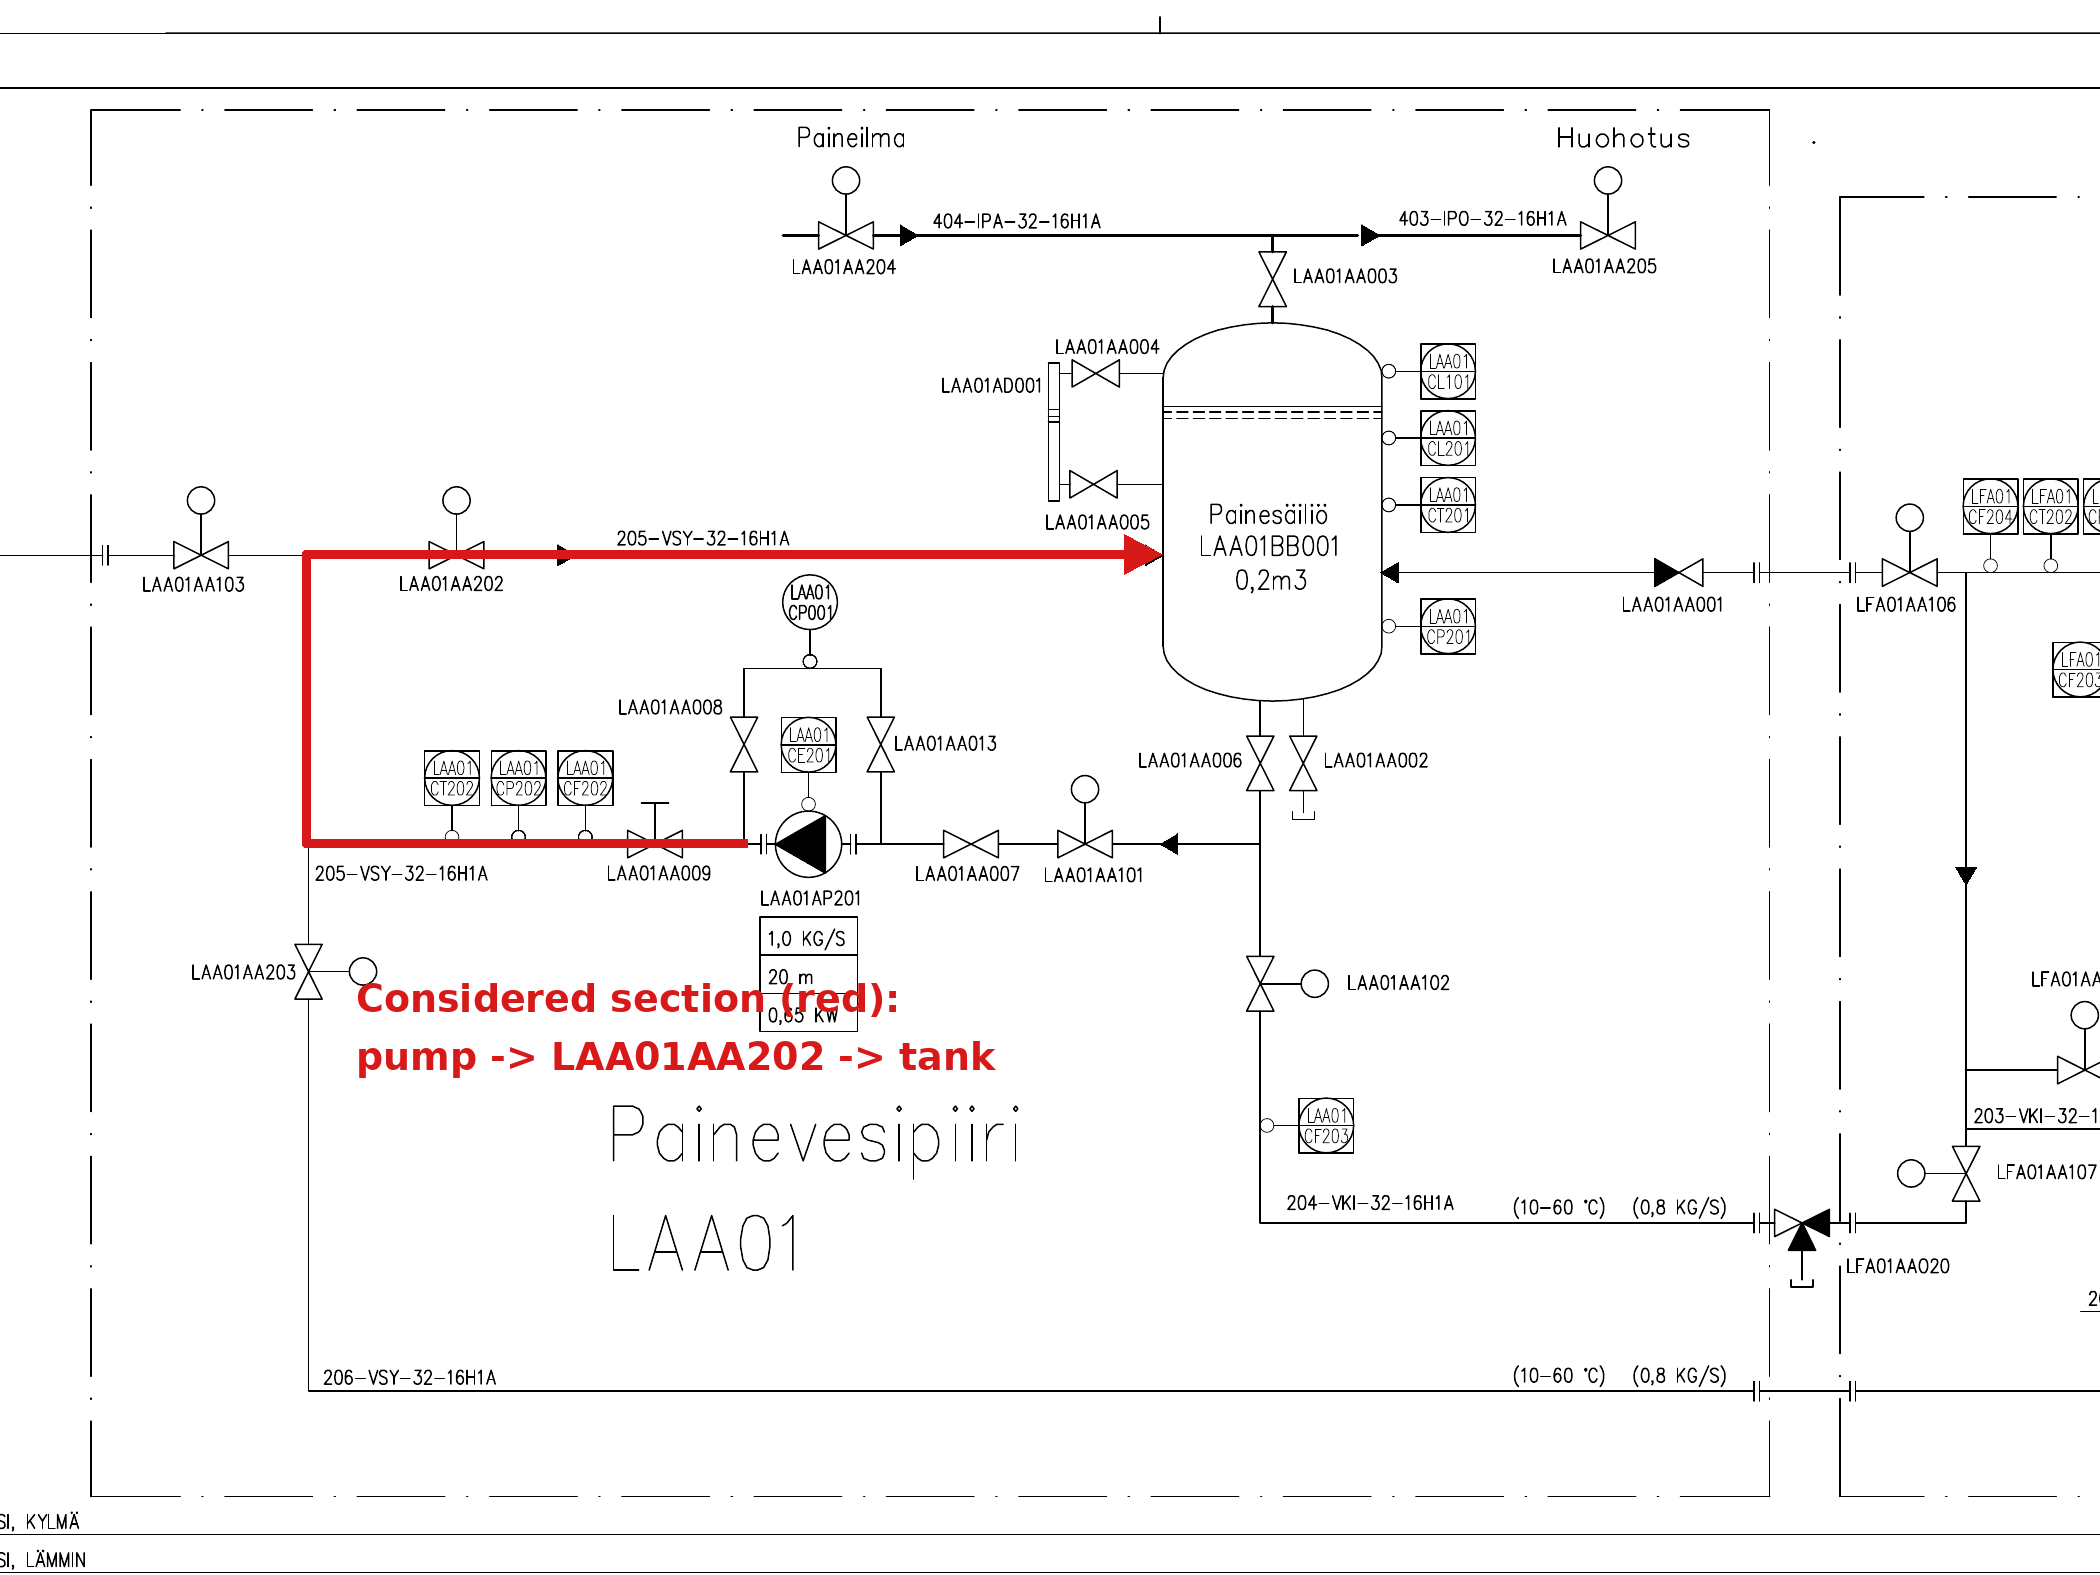
\includegraphics[width=\textwidth]{Pictures/PID_Excerpt_LAA01AA202.png}
    \fignote{Adapted from JAMK University of Applied Sciences (n.d.).}
\end{figure}

\begin{figure}[H]
    \centering
    \caption[Schematic of the section pump $\rightarrow$ valve $\rightarrow$ tank]{Schematic of the section pump $\rightarrow$ valve $\rightarrow$ tank (not to scale, instrument order as in the P\&I diagram)}
    \label{fig:sketch}
    \resizebox{\textwidth}{!}{%
    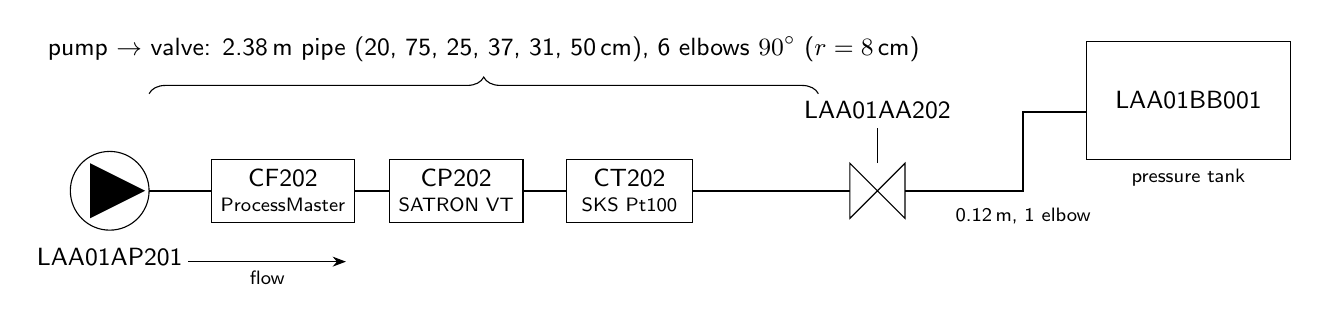
\begin{tikzpicture}[>=Stealth, every node/.style={font=\small}]
        % pump
        \draw (0,0) circle (0.5);
        \fill (-0.25,0.35) -- (-0.25,-0.35) -- (0.45,0) -- cycle;
        \node[below=0.6cm] at (0,0) {LAA01AP201};
        % pipe and instruments
        \draw[thick] (0.5,0) -- (11,0);
        \node[draw,fill=white,minimum width=1.6cm,minimum height=0.8cm,align=center] (cf) at (2.2,0) {CF202\\[-2pt]\scriptsize ProcessMaster};
        \node[draw,fill=white,minimum width=1.6cm,minimum height=0.8cm,align=center] (cp) at (4.4,0) {CP202\\[-2pt]\scriptsize SATRON VT};
        \node[draw,fill=white,minimum width=1.6cm,minimum height=0.8cm,align=center] (ct) at (6.6,0) {CT202\\[-2pt]\scriptsize SKS Pt100};
        % brace over the pump->valve section
        \draw[decorate,decoration={brace,amplitude=6pt,raise=18pt}] (0.5,0.6) -- (9.0,0.6)
            node[midway,above=26pt,align=center] {pump $\rightarrow$ valve: 2.38\,m pipe (20, 75, 25, 37, 31, 50\,cm), 6 elbows $90^\circ$ ($r=8$\,cm)};
        % valve
        \draw[fill=white] (9.4,0.35) -- (9.4,-0.35) -- (10.1,0.35) -- (10.1,-0.35) -- cycle;
        \draw (9.75,0.35) -- (9.75,0.8) node[above] {LAA01AA202};
        % downstream
        \draw[thick] (11,0) -- (11.6,0) -- (11.6,1.0) -- (12.4,1.0);
        \node[below] at (11.6,-0.1) {\scriptsize 0.12\,m, 1 elbow};
        % tank
        \draw (12.4,0.4) rectangle (15.0,1.9);
        \node at (13.7,1.15) {LAA01BB001};
        \node[below] at (13.7,0.4) {\scriptsize pressure tank};
        % flow arrows
        \draw[->] (1.0,-0.9) -- (3.0,-0.9) node[midway,below] {\scriptsize flow};
    \end{tikzpicture}}
\end{figure}

\textbf{Current installation (baseline):}
\begin{itemize}[nosep]
    \item \textbf{Pump:} Kolmeks L-32A/2 centrifugal pump, $105\,\text{mm}$ impeller, 3-phase motor, $50\,\text{Hz}$ (3000\,r/min), DN\,32.
    \item \textbf{Current valve:} Jamesbury 25-716D-31-3600XTZ2 ball valve (DN\,25, PN16), design pressure up to $500\,\text{kPa}$, design temperature up to $120^\circ\text{C}$, design flow range $0$--$0.8\,\text{kg/s}$ according to the device description of LAA01AA202.
    \item \textbf{Current actuator:} AUMA electric part-turn actuator SGR\,04.3.
    \item \textbf{Flow requirement:} design operating flow $q = 0.85\,\text{l/s}$ ($3.06\,\text{m}^3/\text{h}$, $3060\,\text{kg/h}$). This is about 6\,\% above the upper end of the documented design range of the current valve ($0.8\,\text{kg/s}$).
\end{itemize}

% =====================================================================
\section{Calculations and Sizing Methodology}

\subsection{Input Data and Assumptions}
Table~\ref{tab:input} lists the input data. The pipe size was not given in the assignment data and was determined from the P\&I diagram.

\begin{table}[H]
\centering
\caption{Input data}
\label{tab:input}
\small
\begin{tabularx}{\textwidth}{@{}lXl@{}}
\toprule
Quantity & Value & Source \\
\midrule
Medium, temperature & Water, $25^\circ\text{C}$ & Assignment data \\
Design flow $q$ & $0.85\,\text{l/s} = 3.06\,\text{m}^3/\text{h}$ & Assignment data \\
Density $\rho$ / kinematic viscosity $\nu$ & $1000\,\text{kg/m}^3$ / $0.893\,\text{mm}^2/\text{s}$ & Water at $25^\circ\text{C}$ (A3) \\
Vapour pressure $p_v$ & $0.0317\,\text{bar(a)}$ & Nelprof (water, $25^\circ\text{C}$) \\
Pipe (pump to tank) & DN\,32, $d = 32\,\text{mm}$, steel, $\varepsilon = 0.046\,\text{mm}$ & P\&I diagram (JAMK, n.d.) \\
Pump & Kolmeks L-32A/2, $\varnothing 105\,\text{mm}$, $50\,\text{Hz}$ & Kolmeks (2012) \\
Pump head at $q$ / shut-off head & $H = 14\,\text{m}$ / $H_0 = 14.2\,\text{m}$ & Kolmeks (2012), Figure~\ref{fig:pump} \\
Tank pressure $p_{tank}$ & $0.2\,\text{barG}$ & Assumption (A2) \\
Valve candidates & RE-series DN\,25 PN40, M1-series DN\,25 PN40 & Assignment data \\
\bottomrule
\end{tabularx}
\end{table}

\textbf{Assumptions:}
\begin{enumerate}[label=A\arabic*,leftmargin=*,nosep]
    \item Only the section pump $\rightarrow$ valve $\rightarrow$ tank is considered, as required by the assignment. Suction-side losses and static head differences are neglected because the tank is both source and sink.
    \item For the same reason the tank pressure cancels in the pressure balance. $p_{tank} = 0.2\,\text{barG}$ is not given in the assignment; it only defines the absolute pressure level in Nelprof (margin to the vapour pressure), not $\Delta p_{valve}$.
    \item Water properties at $25^\circ\text{C}$; $\rho = 1000\,\text{kg/m}^3$ is used (exact value $997\,\text{kg/m}^3$, difference below 0.3\,\%).
    \item The inner diameter equals the nominal size ($d = 32\,\text{mm}$), as in the pressure drop tables of the Flow Control Manual (Valmet, 2022, p.~154) and in Nelprof (pipeline size 32\,mm). With a real inner diameter of about $35\,\text{mm}$ the velocity would drop to about $0.9\,\text{m/s}$ and the friction losses by roughly $30\,\%$; since the total loss is below $2\,\%$ of the pump head, the effect on the result is negligible.
    \item The design flow is the maximum process flow for the $DP_m$ calculation. $\Delta p_0$ is the pump shut-off pressure (closed valve, no flow, no losses).
    \item LAA01AA009 (safety valve symbol in the P\&I diagram) is a closed side branch in normal operation and causes no flow loss.
\end{enumerate}

\subsection{Pump Curve Analysis}
According to the manufacturer's performance curve of the Kolmeks L-32A/2 pump with a $105\,\text{mm}$ impeller at $50\,\text{Hz}$ (Kolmeks, 2012), the pump delivers $H = 14\,\text{m}$ at $q = 0.85\,\text{l/s}$ and $H_0 \approx 14.2\,\text{m}$ at zero flow (Figure~\ref{fig:pump}). The curve is very flat in this range, so the available pressure hardly depends on the flow.

\begin{figure}[H]
    \centering
    \caption[Pump curve of the Kolmeks L-32A/2 with the operating point]{Pump curve of the Kolmeks L-32A/2 (50\,Hz) with the operating point $q = 0.85\,\text{l/s}$, $H \approx 14\,\text{m}$ marked in red}
    \label{fig:pump}
    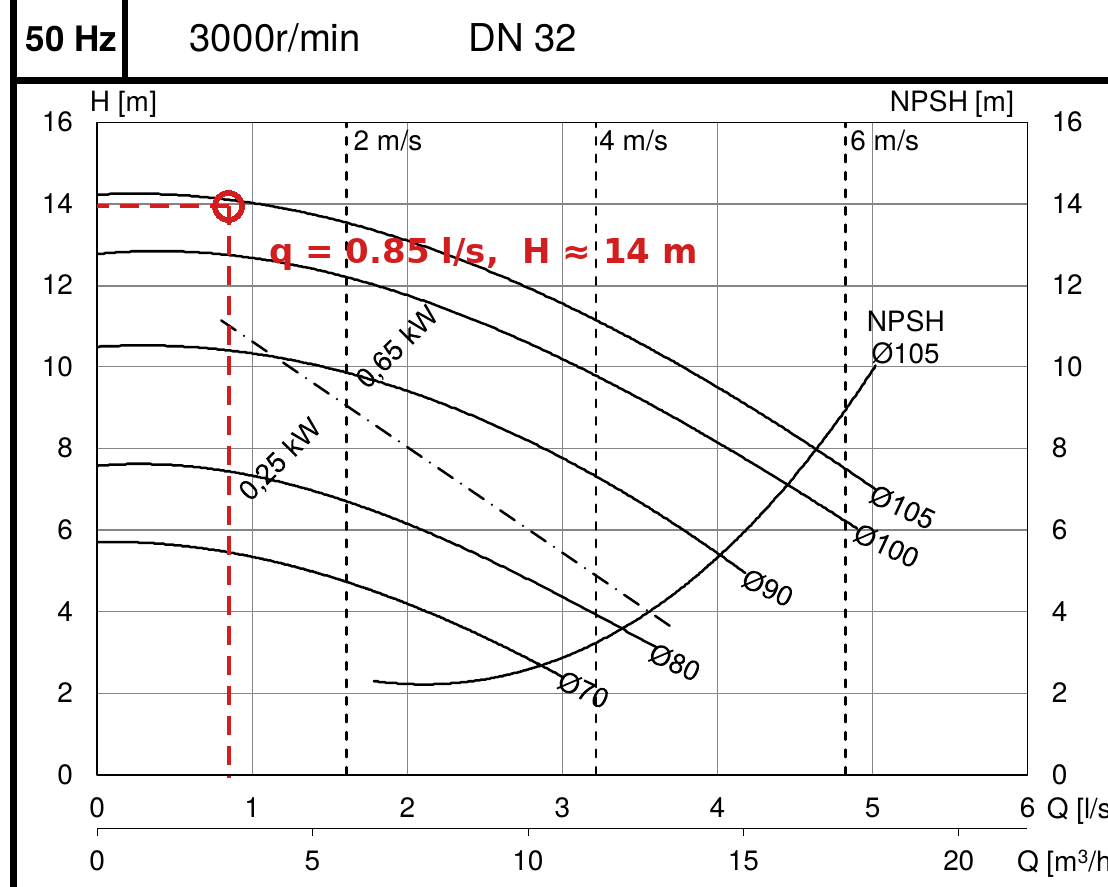
\includegraphics[width=0.75\textwidth]{Pictures/Pump_Curve_Operating_Point.png}
    \fignote{Adapted from Kolmeks (2012).}
\end{figure}

Converting head to pressure ($\rho = 1000\,\text{kg/m}^3$, $g = 9.81\,\text{m/s}^2$):
\begin{equation}
    p_{pump} = \rho g H = 1000 \cdot 9.81 \cdot 14 = 137\,340\,\text{Pa} \approx 1.37\,\text{bar}
\end{equation}
\begin{equation}
    \Delta p_0 = \rho g H_0 = 1000 \cdot 9.81 \cdot 14.2 = 139\,302\,\text{Pa} \approx 1.39\,\text{bar}
\end{equation}
The maximum pressure the pump can provide is therefore the shut-off pressure of about $1.39\,\text{bar}$.

\subsection{Pressure Loss Between Pump and Valve}
All components between the pump discharge and the valve inlet that cause pressure loss were identified from the P\&I diagram and the piping on site (Table~\ref{tab:loss}): $2.38\,\text{m}$ of straight pipe (segments of $20$, $75$, $25$, $37$, $31$ and $50\,\text{cm}$), six $90^\circ$ elbows ($r = 8\,\text{cm}$), the flowmeter CF202, the pressure transmitter CP202 and the temperature sensor CT202. The manual valves LAA01AA006, LAA01AA101 and LAA01AA007 are located on the suction side of the pump and therefore do not belong to this section.

Flow velocity and Reynolds number in the DN\,32 pipe:
\begin{equation}
    v = \frac{4q}{\pi d^2} = \frac{4 \cdot 0.85\cdot 10^{-3}}{\pi \cdot 0.032^2} \approx 1.06\,\text{m/s}, \qquad
    Re = \frac{v d}{\nu} = \frac{1.06 \cdot 0.032}{0.893\cdot 10^{-6}} \approx 3.8\cdot 10^{4}
\end{equation}
The flow is turbulent. The dynamic pressure is $\rho v^2/2 = 559\,\text{Pa}$. The friction factor follows from the Haaland equation (Haaland, 1983) with $\varepsilon/d = 0.046/32 = 1.44\cdot 10^{-3}$:
\begin{equation}
    \frac{1}{\sqrt{f}} = -1.8 \log_{10}\!\left[\left(\frac{\varepsilon/d}{3.7}\right)^{1.11} + \frac{6.9}{Re}\right] \;\Rightarrow\; f \approx 0.026
\end{equation}
The pressure loss of the straight pipe and of the elbows is
\begin{align}
    \Delta p_{pipe} &= f\,\frac{L}{d}\,\frac{\rho v^2}{2} = 0.026 \cdot \frac{2.38}{0.032} \cdot 559 \approx 1.08\,\text{kPa} \\
    \Delta p_{elbows} &= n\,K\,\frac{\rho v^2}{2} = 6 \cdot 0.25 \cdot 559 \approx 0.84\,\text{kPa}
\end{align}
The temperature sensor is the only intrusive element. It is treated as a cylinder in cross flow (drag coefficient $C_D \approx 1.2$) with the well diameter $d_w = 11\,\text{mm}$ from the SKS catalogue (SKS Automaatio, 2015) and a conservative immersion length $L_w = d = 32\,\text{mm}$ (well reaching the opposite wall):
\begin{equation}
    \Delta p_{CT202} = C_D\,\frac{\rho v^2}{2}\,\frac{d_w L_w}{A} = 1.2 \cdot 559 \cdot \frac{0.011 \cdot 0.032}{8.04\cdot 10^{-4}} \approx 0.29\,\text{kPa}
\end{equation}

\begin{table}[H]
\centering
\caption{Pressure loss between pump discharge and valve inlet at $q = 0.85\,\text{l/s}$}
\label{tab:loss}
\small
\begin{tabularx}{\textwidth}{@{}cp{3.6cm}Xrp{2.6cm}@{}}
\toprule
No. & Component & Basis & $\Delta p$ [bar] & Source \\
\midrule
1 & Straight pipe, 2.38\,m, DN\,32 & $f = 0.026$, $L/d = 74.4$ & 0.011 & Haaland (1983) \\
2 & $6\times$ elbow $90^\circ$, $r/d = 2.5$ & $K = 0.25$ each, $\sum K = 1.5$ & 0.008 & Crane Co. (2009) \\
3 & Flowmeter CF202 (ProcessMaster 300) & Electromagnetic, full bore without internals; $K \approx 0$ (assumed) & $\approx 0$ & ABB (n.d.) \\
4 & Pressure transmitter CP202 (SATRON VT) & Pressure tapping, no through-flow, $K \approx 0$ & $\approx 0$ & Satron Instruments (2015) \\
5 & Temperature sensor CT202 (SKS Pt100) & Well $\varnothing 11\,\text{mm}$, $L_w = 32\,\text{mm}$, $C_D = 1.2$ & 0.003 & SKS Automaatio (2015) \\
\midrule
 & \multicolumn{2}{l}{\textbf{Total pump $\rightarrow$ valve}} & \textbf{0.022} & \\
\bottomrule
\end{tabularx}
\end{table}

As a cross-check, the web calculator \textit{Pressure Drop Online} (Pressure Drop Online, n.d.) gives $0.021\,\text{bar}$ for the pipe and the six elbows at $q = 0.85\,\text{l/s}$ (DN\,32), compared with $0.019\,\text{bar}$ from rows 1 and 2 of Table~\ref{tab:loss}. The total loss of about $0.02\,\text{bar}$ is small compared with the pump pressure of $1.37\,\text{bar}$; practically the entire pump pressure remains for the control valve.

Downstream of the valve, the short $0.12\,\text{m}$ pipe with one elbow discharges into the tank:
\begin{equation}
    \Delta p_{down} = 0.026\cdot\frac{0.12}{0.032}\cdot 559 + 0.25\cdot 559 \approx 0.002\,\text{bar}
\end{equation}

\subsection{Pressure Drop Across the Valve and \texorpdfstring{$DP_m$}{DPm}}
Since the static head difference is zero, the pump pressure is dissipated in the pipework and in the valve:
\begin{equation}
    \Delta p_{valve} = p_{pump} - \Delta p_{pump\rightarrow valve} - \Delta p_{down} = 1.373 - 0.022 - 0.002 \approx 1.35\,\text{bar}
\end{equation}
With the assumed tank pressure of $0.2\,\text{barG}$ this gives a valve inlet pressure of $0.2 + 1.373 - 0.022 \approx 1.55\,\text{barG}$ and a valve outlet pressure of about $0.2\,\text{barG}$. The inlet pressure is below the design pressure of the existing valve ($500\,\text{kPa}$) and far below the PN40 rating of the candidates.

According to the Flow Control Manual (Valmet, 2022, p.~23, eq.~10) the process pressure ratio $DP_m$ is the valve pressure drop at the maximum design flow divided by the pressure drop across the closed valve:
\begin{equation}
    DP_m = \frac{\Delta p_m}{\Delta p_0} = \frac{1.35}{1.39} \approx 0.97
\end{equation}
This is far above the rule-of-thumb value $DP_m = 0.30$ for liquid piping (Valmet, 2022, p.~30, eq.~15), which assumes that the valve takes about one third of the total dynamic pressure loss. Here the piping is very short with low losses and the pump curve is flat, so the valve takes almost the entire pump pressure. The consequences for the installed characteristic and gain are discussed in Section~\ref{sec:dpm}.

\subsection{Required Flow Coefficient}
\begin{equation}
    C_v = \frac{q}{N_1\sqrt{\Delta p_{valve}/G_f}} = \frac{3.06\,\text{m}^3/\text{h}}{0.865\cdot\sqrt{1.35/1.0}} \approx 3.04
\end{equation}
with $N_1 = 0.865$ for $q$ in $\text{m}^3/\text{h}$ and $\Delta p$ in bar, and specific gravity $G_f = 1.0$. Nelprof calculates $C_v = 3.05$ (Section~\ref{sec:nelprof}); the small difference comes from rounding.

% =====================================================================
\section{Sizing Results (Nelprof)}
\label{sec:nelprof}
The process data of Table~\ref{tab:nelprof_in} were entered into Valmet Nelprof (Valmet, n.d.) for two DN\,25 PN40 valve alternatives. The complete input and result screens are shown in Appendix~1 (Figures~\ref{fig:setup_re} and~\ref{fig:setup_m1}); the results are summarised in Table~\ref{tab:nelprof_out}.

\begin{table}[H]
\centering
\caption{Nelprof input data}
\label{tab:nelprof_in}
\small
\begin{tabular}{@{}ll@{}}
\toprule
Parameter & Value \\
\midrule
Liquid / flow rate & Water / $0.85\,\text{l/s}$ \\
Inlet temperature & $25^\circ\text{C}$ \\
Inlet pressure / outlet pressure & $1.55\,\text{barG}$ / $0.20\,\text{barG}$ \\
Pressure difference $\Delta p_{valve}$ & $1.35\,\text{bar}$ \\
Vapour pressure & $0.0317\,\text{bar(a)}$ \\
Pipe size inlet / outlet, schedule & $32\,\text{mm}$ / $32\,\text{mm}$, Std \\
\bottomrule
\end{tabular}
\end{table}

\begin{table}[H]
\centering
\caption{Nelprof sizing results at the design operating point}
\label{tab:nelprof_out}
\small
\begin{tabular}{@{}lll@{}}
\toprule
Result & RE-series & M1-series \\
\midrule
Valve, size, pressure class & Segment valve, DN\,25, PN40 & Ball valve, DN\,25, PN40 \\
Trim / maximum capacity & Reduction 2 / $5\,C_v$ & Full bore / $105\,C_v$ \\
Required capacity $C_v$ & 3.05 & 3.05 \\
Travel / opening angle & 82.8\,\% / $80.5^\circ$ & 31.1\,\% / $39.0^\circ$ \\
Recommended travel limits & 3--95\,\% & 5--90\,\% \\
Noise at operating point & 50\,dBA & 41\,dBA \\
Valve outlet / pipe outlet velocity & 1.73\,m/s / 1.06\,m/s & 1.73\,m/s / 1.06\,m/s \\
Choked $\Delta p$ & 2.11\,bar & 2.03\,bar \\
Pressure recovery factor $F_L$ & 0.91 & 0.90 \\
Sizing result status & ok & ok \\
\bottomrule
\end{tabular}
\fignote{Values from the Nelprof result screens (Valmet, n.d.), Figures~\ref{fig:setup_re} and~\ref{fig:setup_m1}.}
\end{table}

All values in Table~\ref{tab:nelprof_out} refer to the design operating point and therefore depend only on the entered flow and pressures, not on the process model used for the installed charts.

\subsection{Alternative 1: RE-Series Segmented Ball Valve}
According to the manufacturer's documentation, the RE-series is a V-port segment valve with an equal-percentage inherent characteristic. For DN\,25 a reduced $C_v$ trim is available to control very low flows (Valmet, 2025). The reduced trim (reduction 2, maximum capacity $5\,C_v$) was selected to match the low required capacity. The required $C_v = 3.05$ agrees with the hand calculation (3.04). The valve operates at 82.8\,\% travel, which is inside the recommended travel limits of 3--95\,\% and uses most of the available stroke. The choked pressure drop of $2.11\,\text{bar}$ is clearly above the actual $\Delta p = 1.35\,\text{bar}$, so the flow is not choked and no heavy cavitation is expected.

\subsection{Alternative 2: M1-Series Standard Ball Valve}
The standard M1-series ball valve (maximum capacity $105\,C_v$) was sized for the same process conditions. It reaches the required $C_v = 3.05$ at only 31.1\,\% travel ($39.0^\circ$), i.e.\ it uses about 3\,\% of its capacity. The noise at the operating point is low (41\,dBA) and the choked pressure drop ($2.03\,\text{bar}$) is also above $1.35\,\text{bar}$. The valve outlet velocity of $1.73\,\text{m/s}$ is the same for both valves (same DN\,25 outlet) and far below the recommended maximum inlet velocity of $10\,\text{m/s}$ for segment and ball valves in continuous duty (Valmet, 2022, p.~65).

% =====================================================================
\section{Graphical Analysis (Nelprof Charts)}
Figures~\ref{fig:inherent} to~\ref{fig:noise} show the Nelprof charts; in each figure the RE-series is displayed on top and the M1-series below. The vertical line marks the design operating point. The installed charts (Figures~\ref{fig:installed} to~\ref{fig:noise}) were calculated by Nelprof with its default process model, which corresponds to $DP_m \approx 0.30$ and not to the calculated $DP_m = 0.97$ (proof in Section~\ref{sec:pressure}). Sections~\ref{sec:inherent} to~\ref{sec:noise} describe the charts as calculated; the effect of the real $DP_m$ is evaluated in Section~\ref{sec:dpm}.

\subsection{Inherent Flow Characteristics}
\label{sec:inherent}
\begin{figure}[H]
    \centering
    \caption{Inherent flow characteristics (top: RE-series, bottom: M1-series)}
    \label{fig:inherent}
    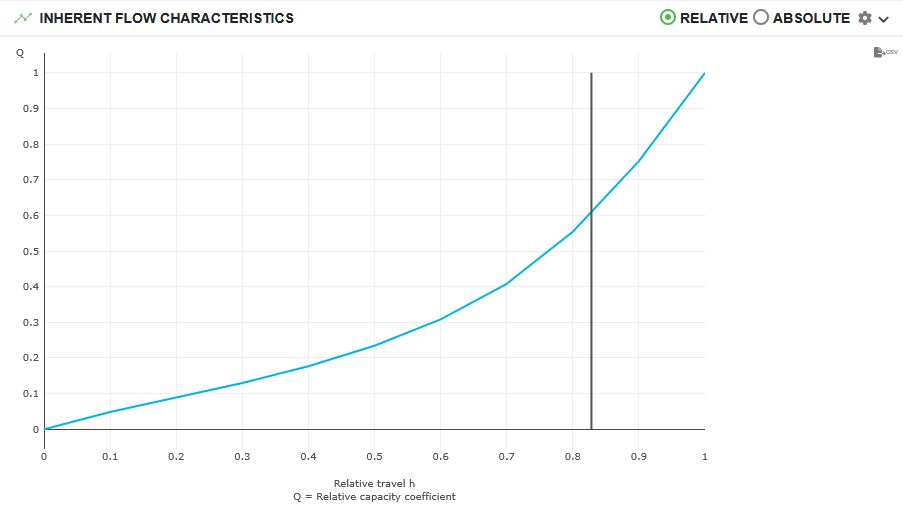
\includegraphics[width=0.82\textwidth]{Pictures Nelprof/RE_InherentFlowCharacteristics_Relative.png}
    \\[0.3cm]
    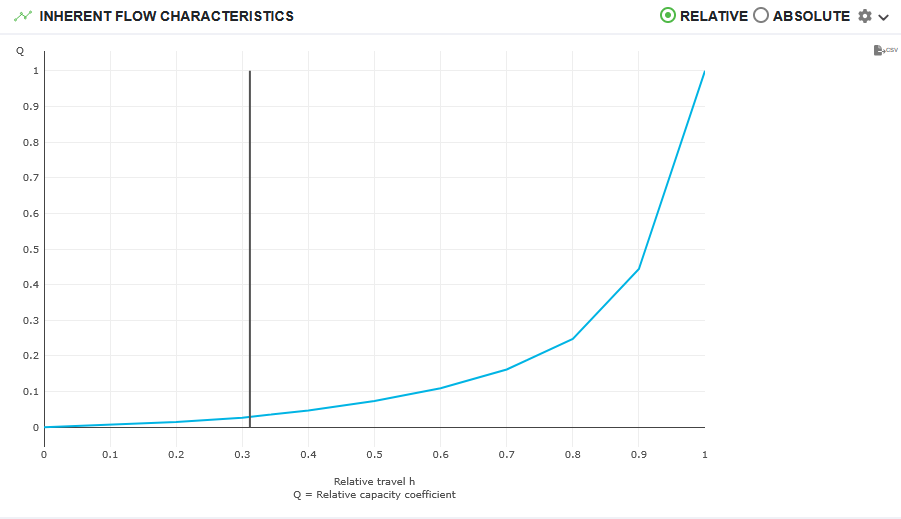
\includegraphics[width=0.82\textwidth]{Pictures Nelprof/M1_InherentFlowCharacteristics_Relative.png}
    \fignote{Screenshots from Nelprof (Valmet, n.d.).}
\end{figure}
Figure~\ref{fig:inherent} shows the relative capacity of the valve as a function of relative travel at constant pressure drop. The RE-series (top) has the equal-percentage characteristic stated by the manufacturer (Valmet, 2025): at 50\,\% travel the relative capacity is about 23\,\%, at 80\,\% travel about 55\,\%. The M1-series (bottom) has a total capacity of $105\,C_v$ and is strongly oversized for a required capacity of about $3\,C_v$. Its curve is flat over the first two thirds of the travel and rises steeply only close to the fully open position. The required capacity is therefore reached at a small opening of about one third of the travel, and most of the capacity of the valve is never used.

\subsection{Installed Flow Characteristics}
\label{sec:installed}
\begin{figure}[H]
    \centering
    \caption{Installed flow characteristics (top: RE-series, bottom: M1-series)}
    \label{fig:installed}
    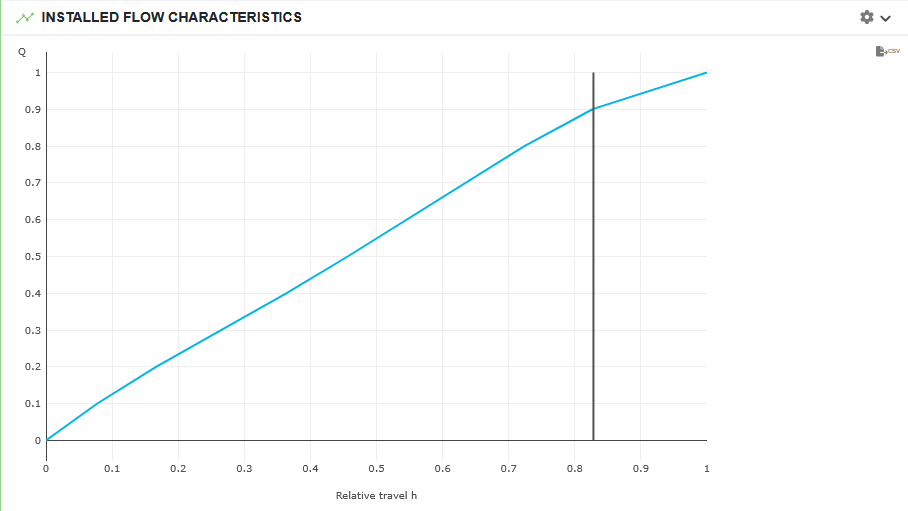
\includegraphics[width=0.82\textwidth]{Pictures Nelprof/RE_InstalledFlowCharacteristics.png}
    \\[0.3cm]
    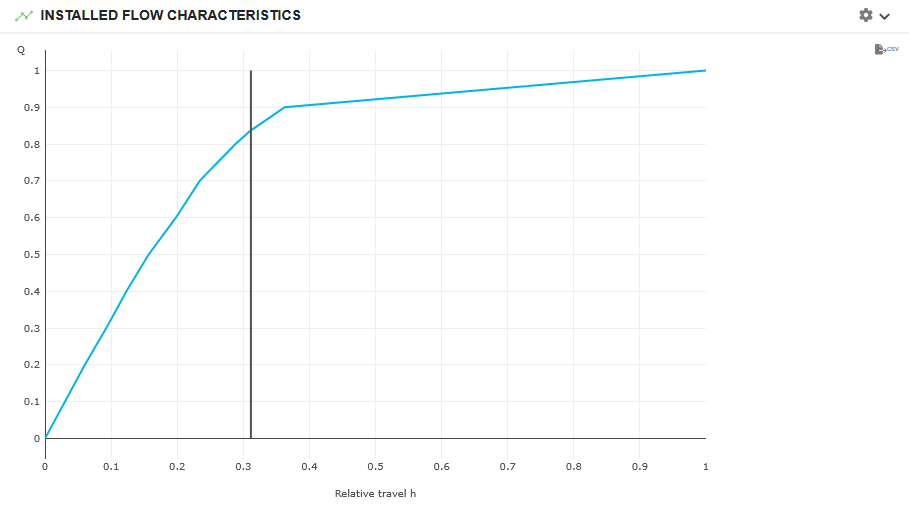
\includegraphics[width=0.82\textwidth]{Pictures Nelprof/M1_InstalledFlowCharacteristics.png}
    \fignote{Screenshots from Nelprof (Valmet, n.d.); calculated with the Nelprof default process model ($DP_m \approx 0.30$).}
\end{figure}
The installed characteristic in Figure~\ref{fig:installed} includes the pressure behaviour of the process. The relative flow $Q = q/q_f$ is the flow divided by the flow through the fully open valve (Valmet, 2022, p.~28). For the RE-series (top) the curve is almost linear: travel 0.5 gives a relative flow of about 0.55 and travel 0.8 about 0.87. At the operating point (82.8\,\% travel) the relative flow is about 0.90, i.e.\ the fully open valve would pass about $0.85/0.90 \approx 0.94\,\text{l/s}$. In this model the RE valve therefore has a flow reserve of only about 10\,\%.

The oversized M1-series (bottom) reaches 80\,\% of its installed flow at about 28\,\% travel and 90\,\% at about 36\,\% travel. Above that the curve is almost flat, because the piping pressure loss in the model then limits the flow. The usable control range is compressed into the first third of the travel and the remaining travel is of no use for this process.

\subsection{Installed Gain}
\label{sec:gain}
\begin{figure}[H]
    \centering
    \caption{Installed gain (top: RE-series, bottom: M1-series)}
    \label{fig:gain}
    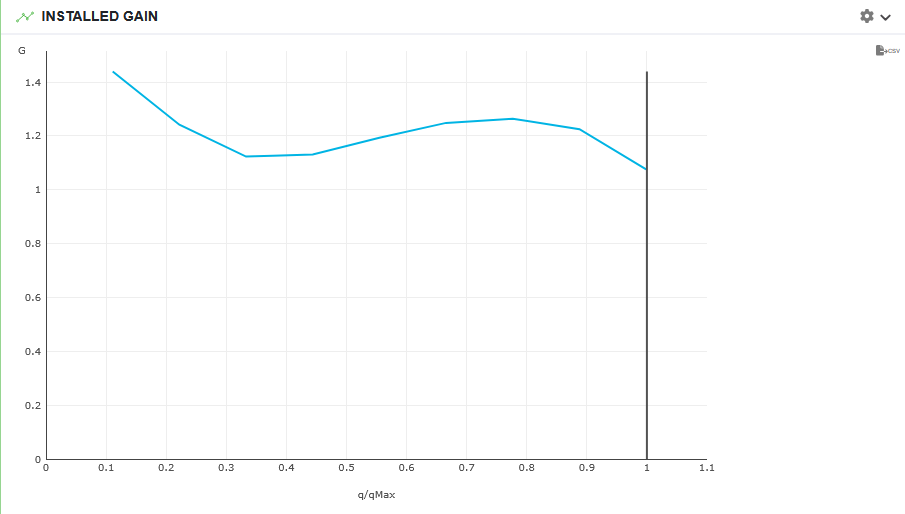
\includegraphics[width=0.82\textwidth]{Pictures Nelprof/RE_InstalledGain.png}
    \\[0.3cm]
    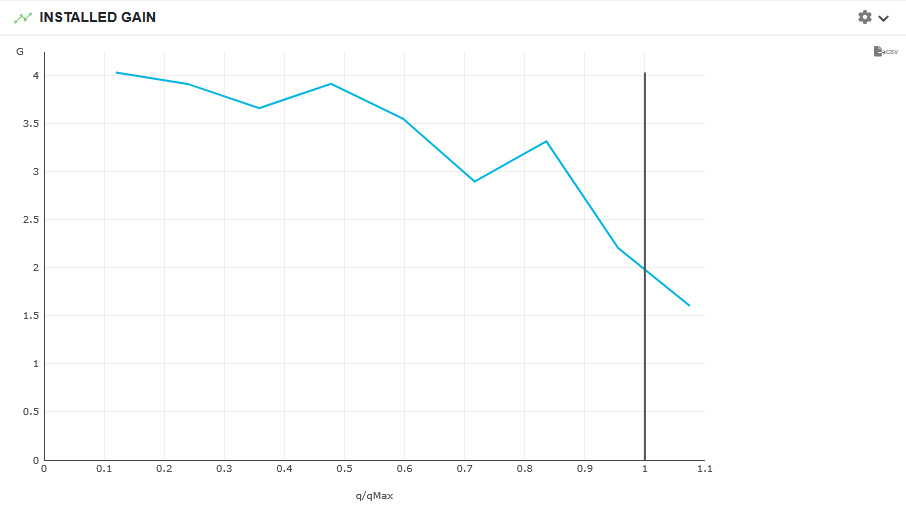
\includegraphics[width=0.82\textwidth]{Pictures Nelprof/M1_InstalledGain.png}
    \fignote{Screenshots from Nelprof (Valmet, n.d.); calculated with the Nelprof default process model ($DP_m \approx 0.30$).}
\end{figure}
The installed gain $G = dQ_p/dh$ describes the sensitivity of the flow to a change in valve position. In Nelprof it is plotted over $q/q_m$, the flow relative to the maximum process flow (Valmet, 2022, p.~28). According to the Flow Control Manual (Valmet, 2022, p.~25, eq.~13 and~14), the change in gain in the operating range should satisfy $G_{max}/G_{min} < 2$ and the gain should not fall below $0.5$.

For the RE-series (Figure~\ref{fig:gain}, top) the gain varies between about 1.07 at the operating point and 1.44 at low flow, so $G_{max}/G_{min} \approx 1.35$. Both criteria are met and the gain is close to 1, i.e.\ a 1\,\% change in travel changes the flow by about 1\,\% of the maximum flow.

For the M1-series (bottom) the gain lies between about 2.0 at the operating point and 4.0 at low flow, so $G_{max}/G_{min} \approx 2.0$, which is exactly at the limit of eq.~13. In addition, the gain is at a high absolute level: a 1\,\% change in travel changes the flow by 2--4\,\%. Since the relative flow error of a control valve is the gain multiplied by the travel error (Valmet, 2022, p.~25), every positioning error of the valve is amplified by a factor of up to four. This promotes oscillation of the control loop and makes tuning of the controller more difficult.

The two curves match the examples in the Flow Control Manual: the M1 gain corresponds to the oversized valve in Figure~19 of the manual (high gain at small flows, poor accuracy and possible hunting), while the RE gain corresponds to the properly sized valve in Figure~20 of the manual with a lower and more constant gain (Valmet, 2022, p.~26).

\subsection{Installed Pressure Level}
\label{sec:pressure}
\begin{figure}[H]
    \centering
    \caption{Installed pressure level (top: RE-series, bottom: M1-series)}
    \label{fig:pressure}
    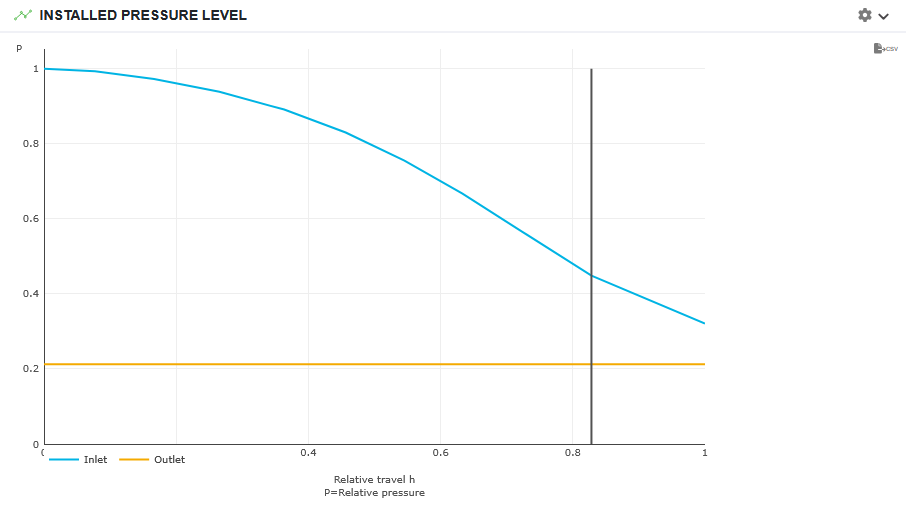
\includegraphics[width=0.82\textwidth]{Pictures Nelprof/RE_InstalledPressureLevel.png}
    \\[0.3cm]
    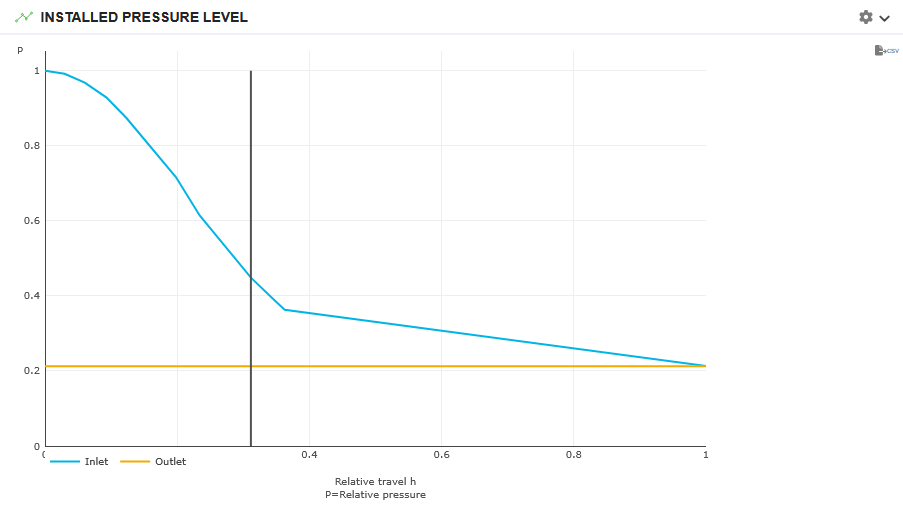
\includegraphics[width=0.82\textwidth]{Pictures Nelprof/M1_InstalledPressureLevel.png}
    \fignote{Screenshots from Nelprof (Valmet, n.d.); calculated with the Nelprof default process model ($DP_m \approx 0.30$).}
\end{figure}
Figure~\ref{fig:pressure} shows the absolute valve inlet and outlet pressure relative to the inlet pressure of the closed valve. With increasing opening the inlet pressure falls from 1.0 to about 0.45 at the operating point for both valves and further to about 0.32 (RE) and 0.21 (M1) at the fully open position. The outlet pressure stays constant at about 0.21. For the M1 the inlet and outlet curves meet at full opening, which means that the valve no longer throttles and the whole pressure is lost in the piping of the model.

The chart also shows which process model Nelprof used. At the operating point the inlet pressure is $1.55\,\text{barG} = 2.56\,\text{bar(a)}$ and its relative value is 0.45, so the closed-valve inlet pressure in the model is $2.56/0.45 \approx 5.7\,\text{bar(a)}$. This is confirmed by the outlet: $1.21\,\text{bar(a)}/5.7\,\text{bar(a)} \approx 0.21$. Thus
\begin{equation}
    \Delta p_{0,\text{Nelprof}} \approx 5.7 - 1.21 \approx 4.5\,\text{bar}, \qquad DP_{m,\text{Nelprof}} \approx \frac{1.35}{4.5} \approx 0.30
\end{equation}
Nelprof therefore used the default value $DP_m \approx 0.30$ (Valmet, 2022, p.~30) instead of the calculated $0.97$, because no second operating point and no $DP_m$ value had been entered. In the real process the inlet pressure can only rise to about $1.59\,\text{barG}$ (pump shut-off pressure plus tank pressure) when the valve closes.

In both cases the pressure downstream of the valve stays far above the vapour pressure of $0.0317\,\text{bar(a)}$, so flashing does not occur (Valmet, 2022, p.~53).

\subsection{Installed Noise}
\label{sec:noise}
\begin{figure}[H]
    \centering
    \caption{Installed hydrodynamic noise (top: RE-series, bottom: M1-series)}
    \label{fig:noise}
    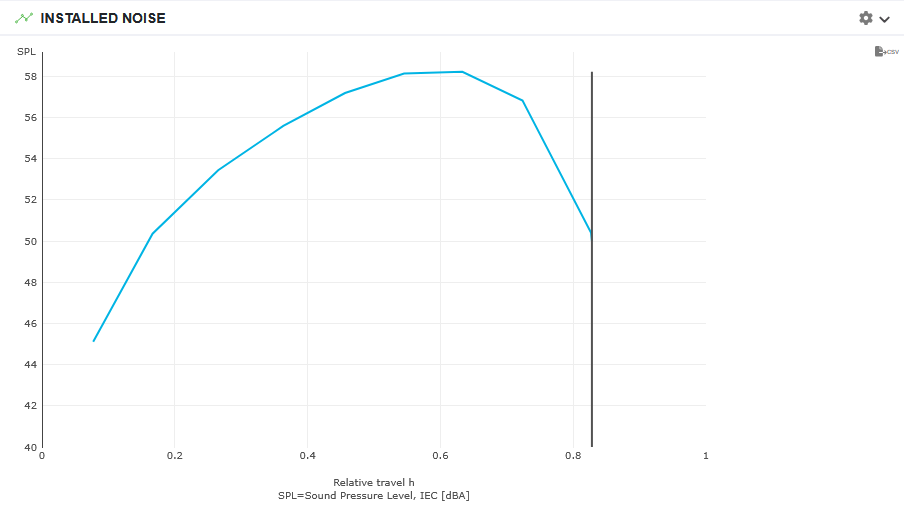
\includegraphics[width=0.82\textwidth]{Pictures Nelprof/RE_InstalledNoise.png}
    \\[0.3cm]
    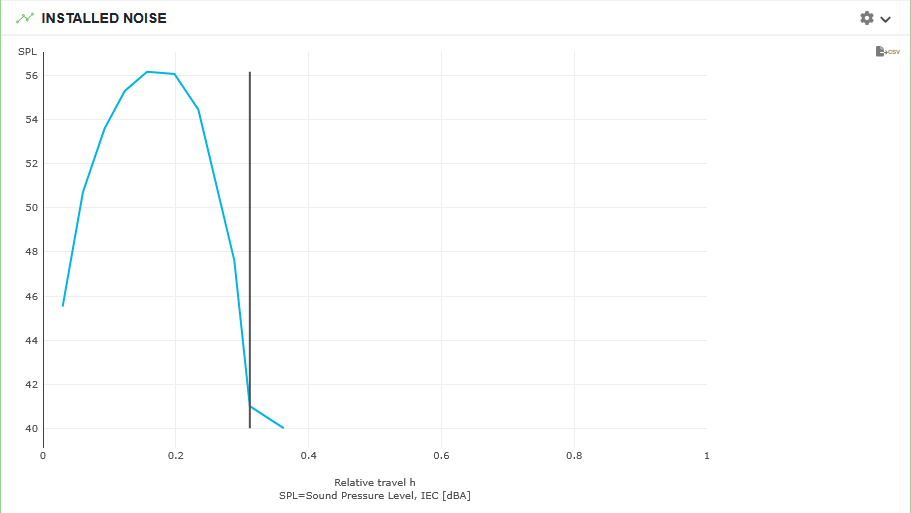
\includegraphics[width=0.82\textwidth]{Pictures Nelprof/M1_InstalledNoise.png}
    \fignote{Screenshots from Nelprof (Valmet, n.d.); calculated with the Nelprof default process model ($DP_m \approx 0.30$).}
\end{figure}
The predicted hydrodynamic noise is a good indicator of cavitation intensity (Valmet, 2022, p.~52). In Figure~\ref{fig:noise} the RE-series peaks at about 58\,dBA at 55--65\,\% travel and reaches 50\,dBA at the operating point. The M1-series peaks at about 56\,dBA at 15--20\,\% travel and reaches 41\,dBA at the operating point. The noise limit for preventing cavitation damage in valves up to DN\,80 is 80\,dB(A) (Valmet, 2022, p.~53, Table~1). Both valves stay more than 20\,dB below this limit, and $\Delta p_{valve} = 1.35\,\text{bar}$ is below the choked pressure drop of both valves. Neither cavitation damage nor flashing is expected. The noise at partial load would be somewhat different with the real $DP_m$, but because the whole pressure difference is only about $1.4\,\text{bar}$, the margin to the limit remains large.

\subsection{Influence of the Real Process Pressure Ratio}
\label{sec:dpm}
The installed charts above were calculated with $DP_m \approx 0.30$, whereas the calculated value for this process is $DP_m = 0.97$. With $DP_m$ close to 1 the pressure drop across the valve stays almost constant over the whole flow range, so the installed characteristic becomes almost identical to the inherent characteristic (Valmet, 2022, pp.~22--24). The installed curves in Figure~\ref{fig:installed} are therefore more linear than they would be in reality.

For the RE-series this means that the installed characteristic would be nearly equal-percentage, like the top curve in Figure~\ref{fig:inherent}. The gain can be estimated from the slope of the inherent curve, divided by the relative capacity at the operating point (about 0.61): between 10\,\% and 30\,\% travel the slope is about 0.4, which gives $G \approx 0.4/0.61 \approx 0.65$; near the operating point the slope is about 2.0, which gives $G \approx 3.3$. The gain would thus change by a factor of about five and the criterion $G_{max}/G_{min} < 2$ (Valmet, 2022, p.~25) would not be met. For the M1-series the same estimate gives a gain of roughly 5--7 at the operating point (slope about 0.2 at a relative capacity of only 0.03), i.e.\ even higher than in Figure~\ref{fig:gain}.

On the other hand, the flow reserve of the RE valve is larger than the 10\,\% read from Figure~\ref{fig:installed}: since the pressure drop hardly decreases when the valve opens, the fully open valve ($5\,C_v$) could pass roughly $5/3.05 \approx 1.6$ times the required capacity, reduced somewhat by the pump curve and the piping losses at higher flow. The 10\,\% value is therefore a conservative estimate.

The non-linear gain of the RE valve can be compensated by characterization, either in the ND9000 digital valve controller or in the controller output, as described in the Flow Control Manual (Valmet, 2022, pp.~32--34). With such a correction the installed characteristic becomes approximately linear. For the M1 valve characterization does not help much, because the whole control range is compressed into a small part of the stroke, where travel errors are amplified strongly.

% =====================================================================
\section{Comparative Evaluation and Conclusions}

\subsection{Valve Performance Comparison}
Table~\ref{tab:compare} summarises the comparison of the two alternatives.

\begin{table}[!htb]
\centering
\caption{Comparison of the RE-series and M1-series valves}
\label{tab:compare}
\small
\begin{tabularx}{\textwidth}{@{}lXX@{}}
\toprule
Criterion & RE-series (reduced trim, $5\,C_v$) & M1-series ($105\,C_v$) \\
\midrule
Travel / opening at design flow & 82.8\,\% / $80.5^\circ$ & 31.1\,\% / $39.0^\circ$ \\
Use of capacity & about 60\,\% & about 3\,\% \\
Installed gain (Nelprof) & 1.07--1.44, $G_{max}/G_{min} \approx 1.35$ (criterion met) & 2.0--4.0, $G_{max}/G_{min} \approx 2.0$ (at the limit) \\
Noise at operating point / peak & 50\,dBA / 58\,dBA & 41\,dBA / 56\,dBA \\
Choked $\Delta p$ vs.\ $\Delta p = 1.35\,\text{bar}$ & 2.11\,bar, not choked & 2.03\,bar, not choked \\
Cavitation / flashing & no / no & no / no \\
Flow reserve & about 10\,\% (Nelprof model), larger with real $DP_m$ & large, but in the flat part of the curve \\
\bottomrule
\end{tabularx}
\end{table}

The M1-series ball valve, which corresponds to the currently installed valve type, offers tight shut-off and a very high maximum capacity. For a throttling duty at about $3\,C_v$ this capacity is a disadvantage (JAMK University of Applied Sciences, 2024): the valve uses only about one third of its stroke, reaches 90\,\% of its installed flow at about 36\,\% travel and has a high installed gain of up to 4. This leaves little resolution for the controller.

The RE-series segmented ball valve with reduced trim matches the required capacity much better. It uses most of its stroke and has an installed gain close to 1 that fulfils the criteria of the Flow Control Manual. Two limitations have to be noted. First, in the Nelprof model the flow reserve at the design flow is only about 10\,\%; with the real $DP_m$ the reserve is larger, but a flow requirement clearly above $0.85\,\text{l/s}$ should be checked again. Second, because of the real $DP_m \approx 0.97$ the installed characteristic will be close to equal-percentage and the gain will vary more than in Figure~\ref{fig:gain}; a characterization in the valve controller or in the control system is therefore recommended (Section~\ref{sec:dpm}).

\subsection{Product Documentation of the Selected Valve}
The manufacturer's documentation (Valmet, 2025) describes the RE-series as an integrally flanged V-port segment valve in quarter-turn design with an equal-percentage inherent characteristic. The reduced $C_v$ trim is available for DN\,25 valves only and is intended for very low flows, which matches the required capacity of about $3\,C_v$. Standard units are supplied with pneumatic diaphragm or cylinder actuators and ND9000 intelligent valve controllers, which also offer the characterization function mentioned in Section~\ref{sec:dpm}.

\subsection{Actuator}
The installed AUMA SGR\,04.3 is an electric part-turn actuator. The manufacturer's standard configuration for the RE-series uses a pneumatic actuator with an ND9000 valve controller (Valmet, 2025). Changing the actuator is a secondary recommendation; the valve selection does not depend on it.

\subsection{Final Verdict}
Based on the process data, the pressure loss calculation between pump and valve ($\Delta p_{valve} = 1.35\,\text{bar}$, $DP_m = 0.97$, $C_v \approx 3.05$) and the Nelprof analysis, the \textbf{RE-series segmented ball valve (DN\,25, PN40, reduced trim with $5\,C_v$)} is more suitable for this application than the M1-series ball valve. It has a suitable capacity, uses most of its stroke and has a stable installed gain, without cavitation or flashing. The M1-series is strongly oversized, uses only about one third of its stroke and has a high installed gain. For the RE valve a characterization in the ND9000 or in the controller is recommended, and the limited flow reserve should be kept in mind if the flow requirement increases.

% =====================================================================
\section*{Declaration on the Use of Artificial Intelligence}
\addcontentsline{toc}{section}{Declaration on the Use of Artificial Intelligence}
In accordance with the JAMK guidelines, generative AI (Claude, Anthropic) was used as a support tool. It was used for language checking, for formatting the LaTeX document according to the JAMK reporting template and for reviewing the calculation approach (pressure balance, $DP_m$ definition) and the consistency between the calculations, the Nelprof results and the text. The pipe friction calculation, the component losses, the pressure drop across the valve, $DP_m$ and $C_v$ (Section~3) were calculated and checked by the author; the pipe loss was cross-checked with \textit{Pressure Drop Online}. All sizing was performed by the author in Nelprof, the values read from the Nelprof charts were checked by the author, and the interpretation of the results and the valve selection are the author's own. The author is fully responsible for the technical content.

% =====================================================================
\clearpage
\section*{References}
\addcontentsline{toc}{section}{References}
\begingroup
\setlength{\parindent}{-1.25cm}
\setlength{\leftskip}{1.25cm}
\setlength{\parskip}{8pt}
\raggedright
ABB. (n.d.). \textit{ProcessMaster FEP300 electromagnetic flowmeter} (Data sheet DS/FEP300-EN, Rev. K). \url{https://library.e.abb.com/public/5996486236d6463ab3375fb48033fd17/DS_FEP300_EN_K.pdf}

Crane Co. (2009). \textit{Flow of fluids through valves, fittings, and pipe} (Technical Paper No. 410). Crane Co.

Haaland, S. E. (1983). Simple and explicit formulas for the friction factor in turbulent pipe flow. \textit{Journal of Fluids Engineering, 105}(1), 89--90. \url{https://doi.org/10.1115/1.3240948}

JAMK University of Applied Sciences. (n.d.). \textit{Process diagram 35899, rev. 7} [P\&I diagram]. Field Devices and Instrumentation course material, JAMK Moodle.

JAMK University of Applied Sciences. (2024). \textit{Valve structures and control valves} [Learning material]. Field Devices and Instrumentation course material, JAMK Moodle.

Kolmeks. (2012). \textit{Pump performance curve: L-32A/2, 50/60 Hz (105 mm impeller)} [Data sheet].

Pressure Drop Online. (n.d.). \textit{Pressure drop online-calculator} [Web application]. Retrieved 2.10.2026 from \url{https://www.pressure-drop.com/Online-Calculator/}

Satron Instruments. (2015). \textit{SATRON VT painel\"ahetin} [Data sheet].

SKS Automaatio. (2015). \textit{L\"amp\"otila-anturi: Valmistusohjelma ja anturityypit} [Data sheet].

Valmet. (n.d.). \textit{Nelprof sizing and selection software} [Computer software]. Retrieved 2.10.2026 from \url{https://www.valmet.com/flowcontrol/valves/valve-sizing-selection-software-nelprof/}

Valmet. (2022). \textit{Flow control manual} (6th ed.). Neles Finland Oy.

Valmet. (2025). \textit{Neles V-port segment valve RE-series} (Brochure 3R24EN). \url{https://www.valmet.com/globalassets/sharepoint/imported/3r24en.pdf}
\endgroup

% =====================================================================
\clearpage
\section*{Appendices}
\addcontentsline{toc}{section}{Appendices}
\subsection*{Appendix 1. Nelprof Setup and Results}
\addcontentsline{toc}{subsection}{Appendix 1. Nelprof Setup and Results}
\begin{figure}[H]
    \centering
    \caption{Nelprof input data and results, RE-series}
    \label{fig:setup_re}
    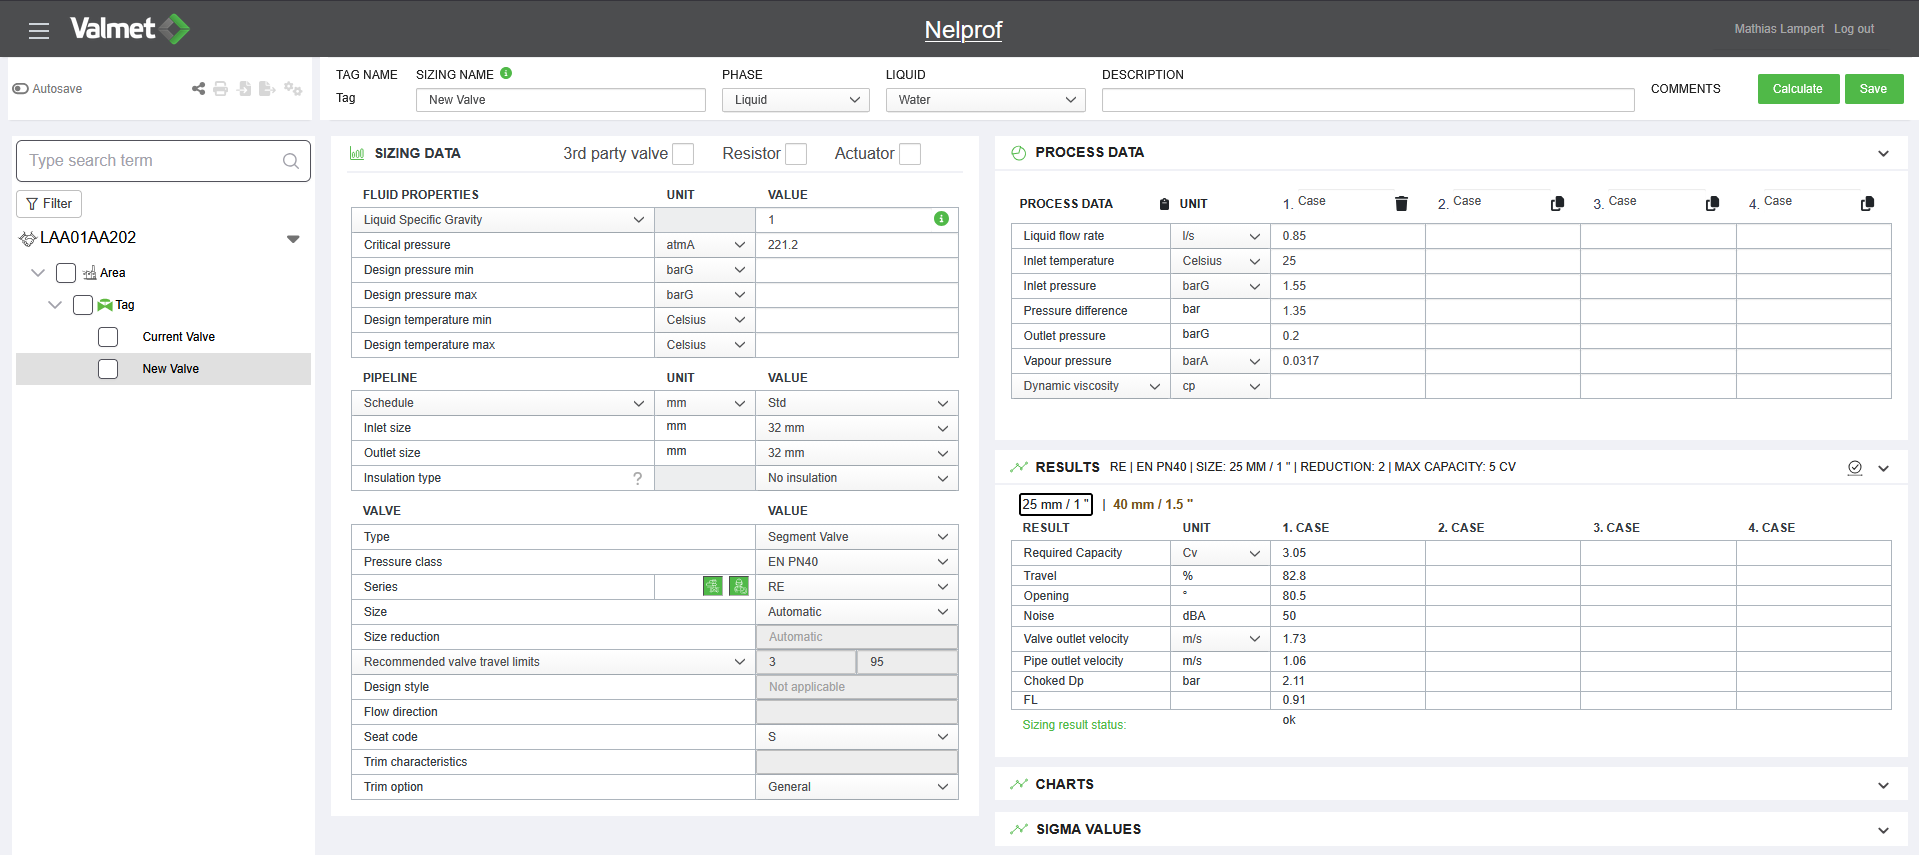
\includegraphics[width=\textwidth]{Pictures Nelprof/RE_Nelprof_Setup.png}
    \fignote{Screenshot from Nelprof (Valmet, n.d.).}
\end{figure}
\begin{figure}[H]
    \centering
    \caption{Nelprof input data and results, M1-series}
    \label{fig:setup_m1}
    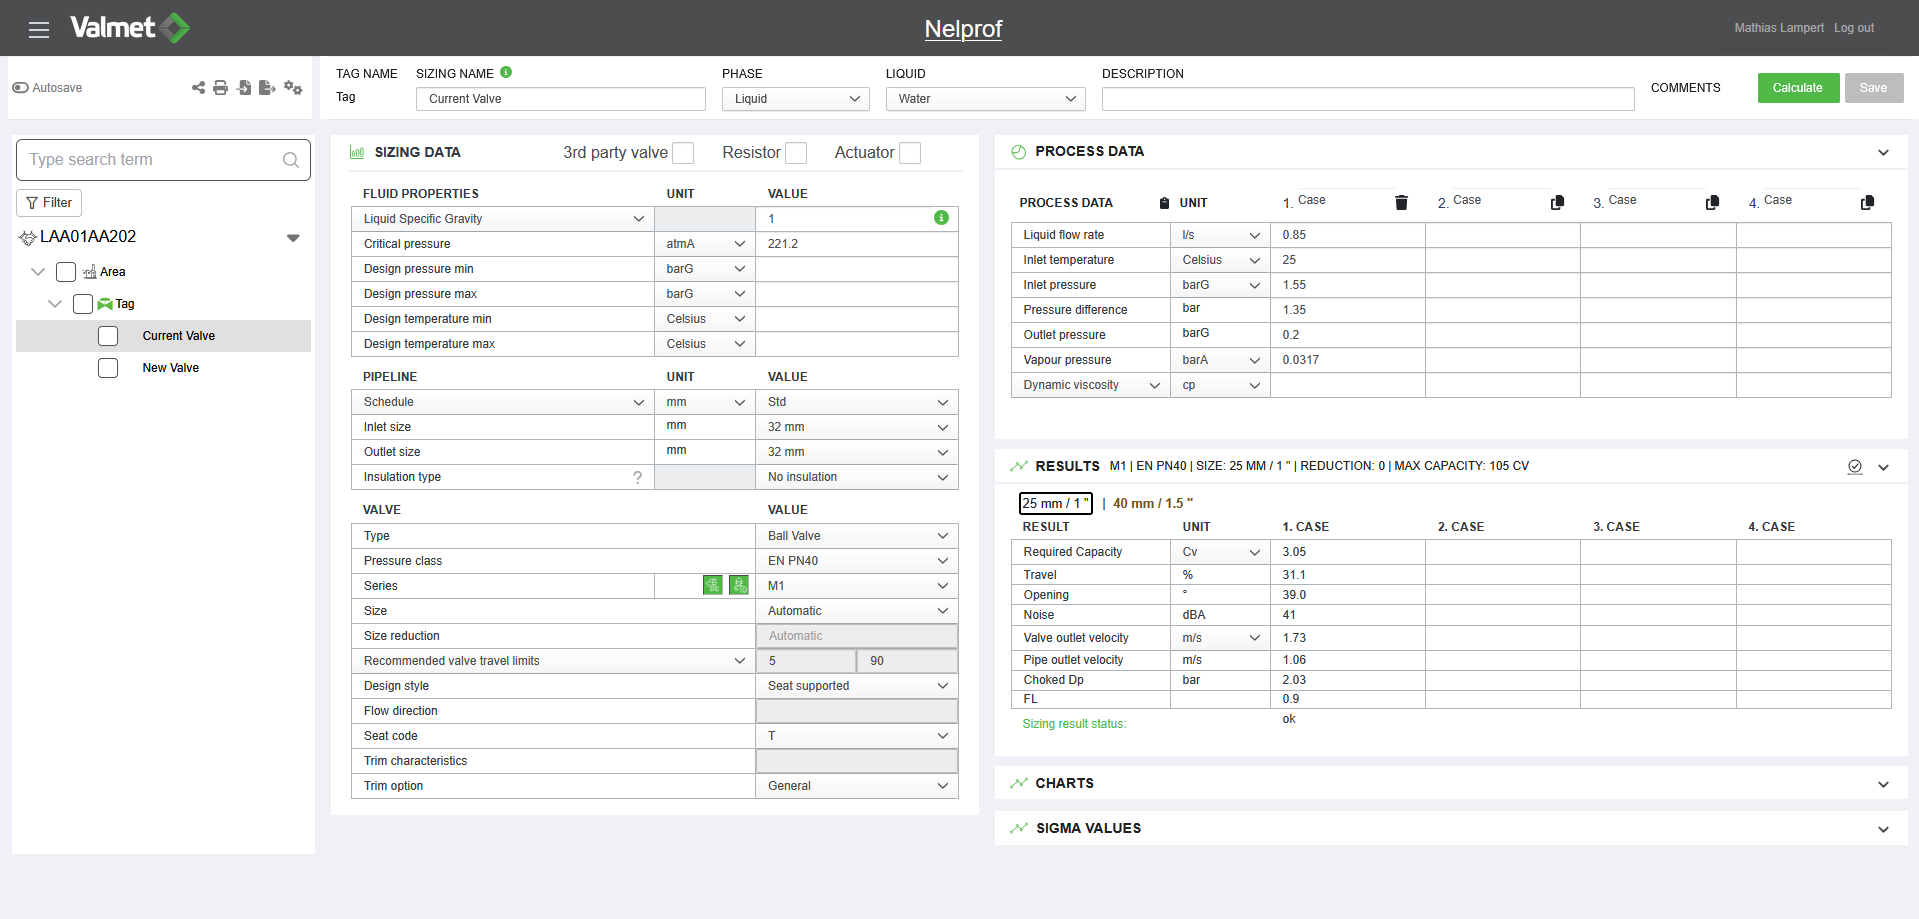
\includegraphics[width=\textwidth]{Pictures Nelprof/M1_Nelprof_Setup.png}
    \fignote{Screenshot from Nelprof (Valmet, n.d.).}
\end{figure}

\end{document}
